\documentclass[a4 paper]{article}
% Set target color model to RGB
\usepackage[inner=1.5cm,outer=1.5cm,top=2.5cm,bottom=2.5cm]{geometry}
\usepackage{setspace}
\usepackage[rgb]{xcolor}
\usepackage{verbatim}
\usepackage{amsgen,amsmath,amstext,amsbsy,amsopn,tikz,amssymb,tkz-linknodes}
\usepackage{fancyhdr}
\usepackage[colorlinks=true, urlcolor=blue,  linkcolor=blue, citecolor=blue]{hyperref}
\usepackage[colorinlistoftodos]{todonotes}
\usepackage{rotating}
%\usetikzlibrary{through,backgrounds}
\hypersetup{%
pdfauthor={Arman Shokrollahi},%
pdftitle={Homework},%
pdfkeywords={Tikz,latex,bootstrap,uncertaintes},%
pdfcreator={PDFLaTeX},%
pdfproducer={PDFLaTeX},%
}
%\usetikzlibrary{shadows}
\usepackage[francais]{babel}
\usepackage{booktabs}
\newcommand{\ra}[1]{\renewcommand{\arraystretch}{#1}}

      \newtheorem{thm}{Theorem}[section]
      \newtheorem{prop}[thm]{Proposition}
      \newtheorem{lem}[thm]{Lemma}
      \newtheorem{cor}[thm]{Corollary}
      \newtheorem{defn}[thm]{Definition}
      \newtheorem{rem}[thm]{Remark}
      \numberwithin{equation}{section}

\newcommand{\homework}[6]{
   \pagestyle{myheadings}
   \thispagestyle{plain}
   \newpage
   \setcounter{page}{1}
   \noindent
   \begin{center}
   \framebox{
      \vbox{\vspace{2mm}
    \hbox to 6.28in { {\bf\hfill} }
       \vspace{6mm}
       \hbox to 6.28in { {\Large \hfill #1 (#2)  \hfill} }
       \vspace{6mm}
       \hbox to 6.28in { {\it Instructor: #3 \hfill Student: #5} }
       %\hbox to 6.28in { {\it TA: #4  \hfill #6}}
      \vspace{2mm}}
   }
   \end{center}
   \markboth{#5 -- #1}{#5 -- #1}
   \vspace*{4mm}
}

\newcommand{\bbF}{\mathbb{F}}
\newcommand{\bbX}{\mathbb{X}}
\newcommand{\bI}{\mathbf{I}}
\newcommand{\bX}{\mathbf{X}}
\newcommand{\bY}{\mathbf{Y}}
\newcommand{\bepsilon}{\boldsymbol{\epsilon}}
\newcommand{\balpha}{\boldsymbol{\alpha}}
\newcommand{\bbeta}{\boldsymbol{\beta}}
\newcommand{\0}{\mathbf{0}}

\begin{document}
\homework{Actividad \#8}{C\'omputo Simb\'olico con Maxima}{Carlos Liz\'arraga Celaya}{}{Antonio Cota Rodr\'iguez}{}

\section*{Introducci\'on}
\setlength{\parindent}{1.2em}
\subsection*{wxMaxima}
El sistema de \'algebra computacional Maxima es un motor de c\'alculo simb\'olico escrito en lenguaje Lisp publicado bajo licencia GNU GPL.\\

Cuenta con un amplio conjunto de funciones para hacer manipulaci\'on simb\'olica de polinomios, matrices, funciones racionales, integraci\'on, derivaci\'on, manejo de gr\'aficos en 2D y 3D, manejo de n\'umeros de coma flotante muy grandes, expansi\'on en series de potencias y de Fourier, entre otras funcionalidades. Adem\'as tiene un depurador a nivel de fuente para el c\'odigo de Maxima.\\

Maxima est\'a basado en el sistema original de Macsyma desarrollado por MIT en los años 70. Es bastante fiable, tiene un buen recolector de basura, por lo que no desperdicia memoria. Viene con cientos de auto pruebas (test-suite).

\section*{Actividad}

Durante toda la actividad se mostrar\'an im\'agenes para evidenciar el trabajo hecho, cada imagen cuenta con su respectiva descripci\'on de lo que se realiz\'o paso por paso. La din\'amica es la siguiente; se mostrar\'a la imagen y si el resultado dio una gr\'afica se presentar\'a abajo del c\'odigo.

\section*{Cap\'itulo 2}
\subsection*{2.1 Vectores y \'Algebra lineal}


\begin{figure}[!ht]
  \centering
      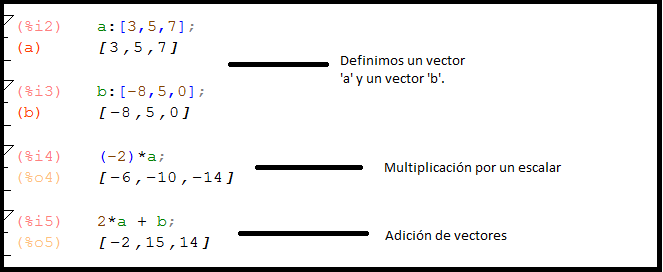
\includegraphics[width=6.6cm, height=2.7cm]{SumaProducto.png}
  \caption{Suma y producto por un escalar}
\end{figure}

\begin{figure}[!ht]
  \centering
      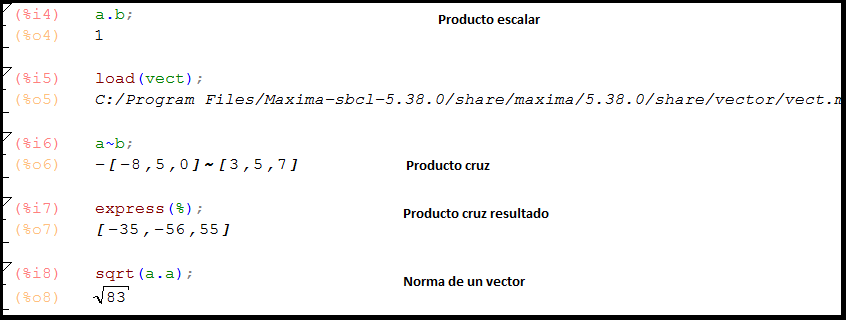
\includegraphics[width=8.4cm, height=3.2cm]{PuntoCruzNorma.png}
  \caption{Producto cruz, punto y norma de un vector}
\end{figure}
\newpage

\begin{figure}[!ht]
  \centering
      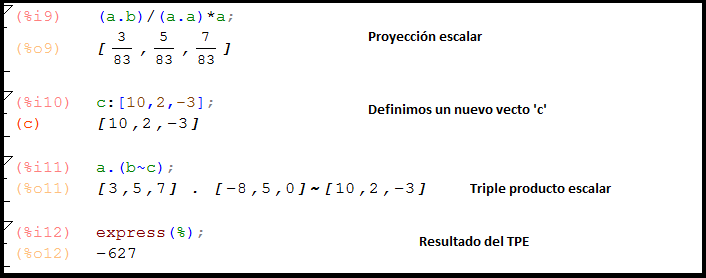
\includegraphics[width=7.1cm, height=2.7cm]{ProyeccionTPE.png}
  \caption{Proyecci\'on escalar y triple producto escalar}
\end{figure}

%--------------------------------------------------------------------

\subsection*{2.2 Lineas, planos y superficies cu\'adricas}

\begin{figure}[!ht]
  \centering
      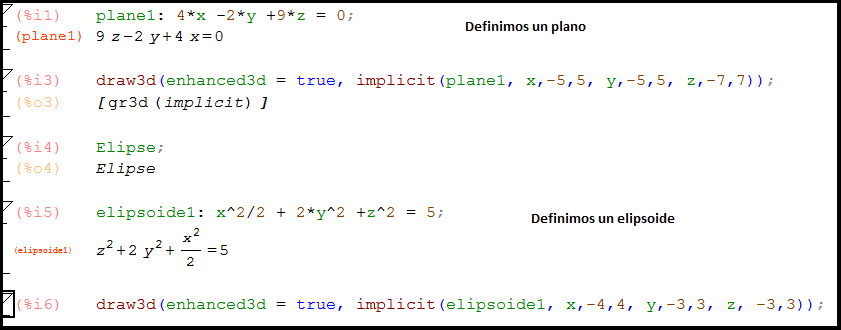
\includegraphics[width=8.4cm, height=3.3cm]{PlanoElipsoide.png}
  \caption{Ecuaci\'on de un plano y una elipsoide}
\end{figure}

\begin{figure}[!ht]
  \centering
      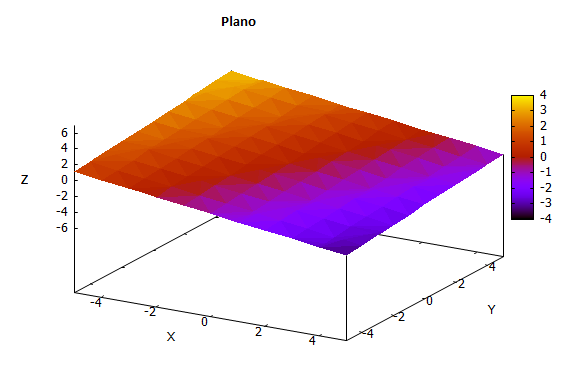
\includegraphics[width=5.7cm, height=3.6cm]{Plano1.png}
  \caption{Gr\'afica del plano}
\end{figure}

\begin{figure}[!ht]
  \centering
      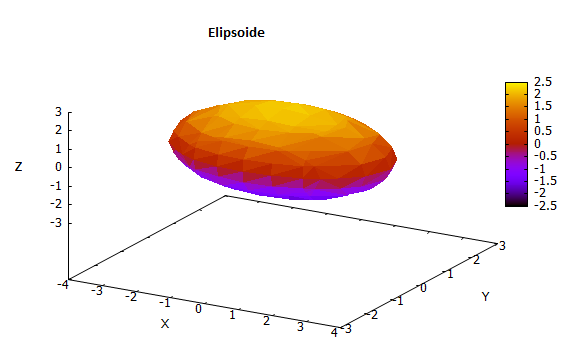
\includegraphics[width=5.7cm, height=3.6cm]{Elipsoide1.png}
  \caption{Gr\'afica de la elipsoide}
\end{figure}
\newpage
\begin{figure}[!ht]
  \centering
      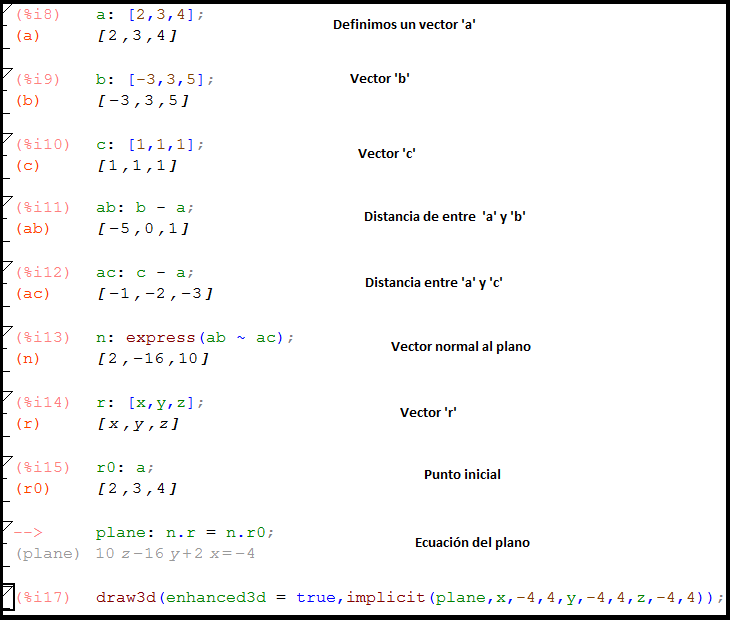
\includegraphics[width=7.3cm, height=6.2cm]{EcuacionDelPlano.png}
  \caption{Ecuaci\'on de un plano a partir de tres puntos}
\end{figure}

\begin{figure}[!ht]
  \centering
      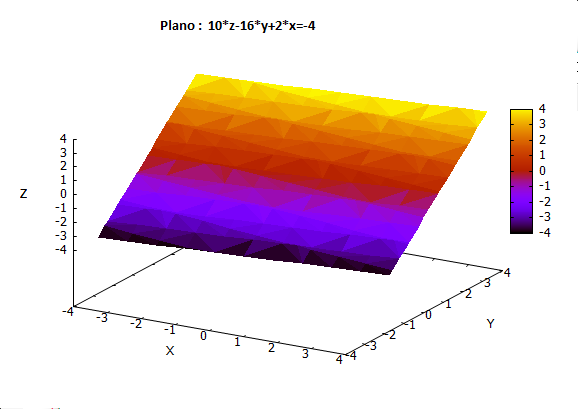
\includegraphics[width=5.8cm, height=4.1cm]{Plano2.png}
  \caption{Plano dado 3 puntos}
\end{figure}

\begin{figure}[!ht]
  \centering
      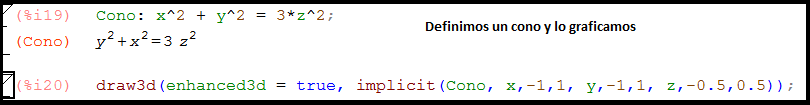
\includegraphics[width=8.1cm, height=1.1cm]{EcuacionCono.png}
  \caption{Cono en Maxima}
\end{figure}

\begin{figure}[!ht]
  \centering
      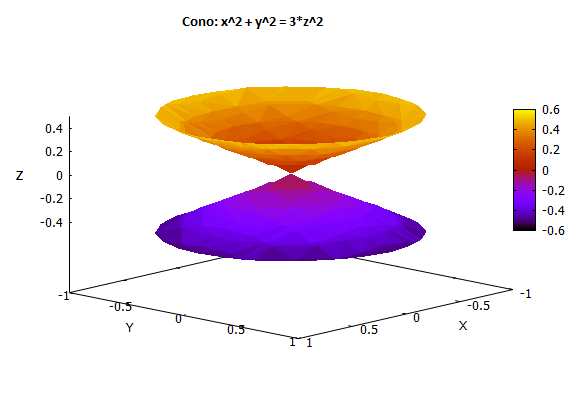
\includegraphics[width=5.7cm, height=4.1cm]{Cono1.png}
  \caption{Gr\'afica del cono}
\end{figure}

%--------------------------------------------------------------------

\subsection*{2.3 Funciones vectoriales}
\newpage

\begin{figure}[!ht]
  \centering
      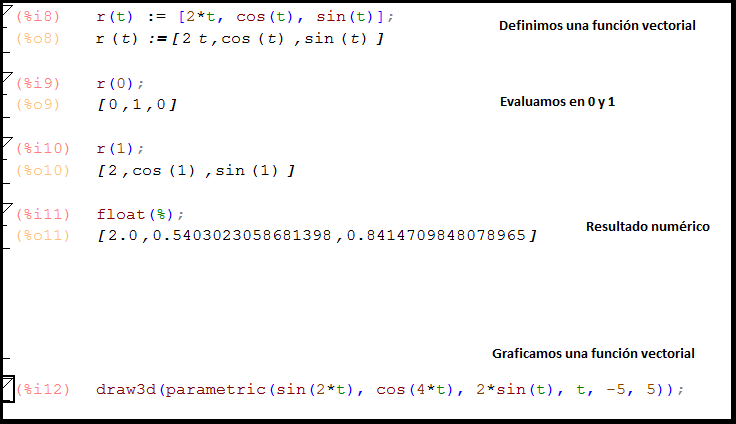
\includegraphics[width=7.3cm, height=4.2cm]{FuncionVectorial.png}
  \caption{Funci\'on vectorial evaluada}
\end{figure}

\begin{figure}[!ht]
  \centering
      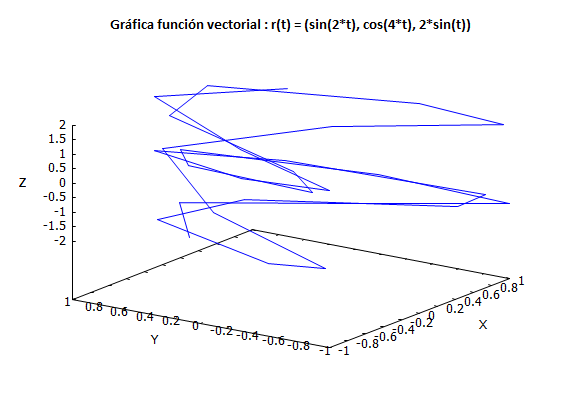
\includegraphics[width=5.7cm, height=4.0cm]{GraficaFuncionVectorial.png}
  \caption{Gr\'afica de la funci\'on vectorial}
\end{figure}

\begin{figure}[!ht]
  \centering
      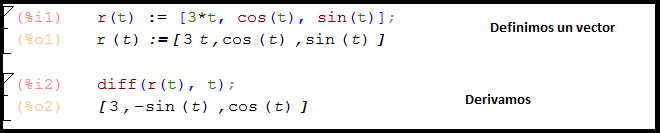
\includegraphics[width=6.6cm, height=1.3cm]{Derivada.png}
  \caption{Derivada de la funci\'on vectorial}
\end{figure}
\newpage
\begin{figure}[!ht]
  \centering
      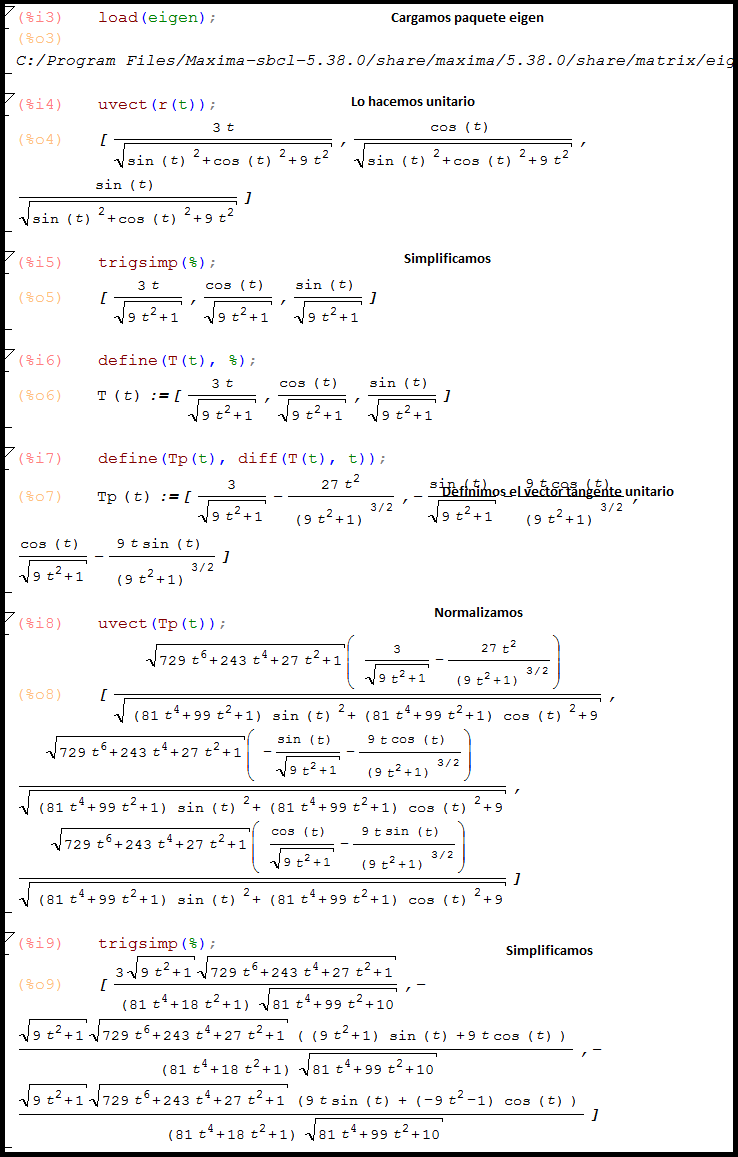
\includegraphics[width=10.4cm, height=16 cm]{VectorTangenteUnitario.png}
  \caption{Vector tangente unitario}
\end{figure}

\newpage

\begin{figure}[!ht]
  \centering
      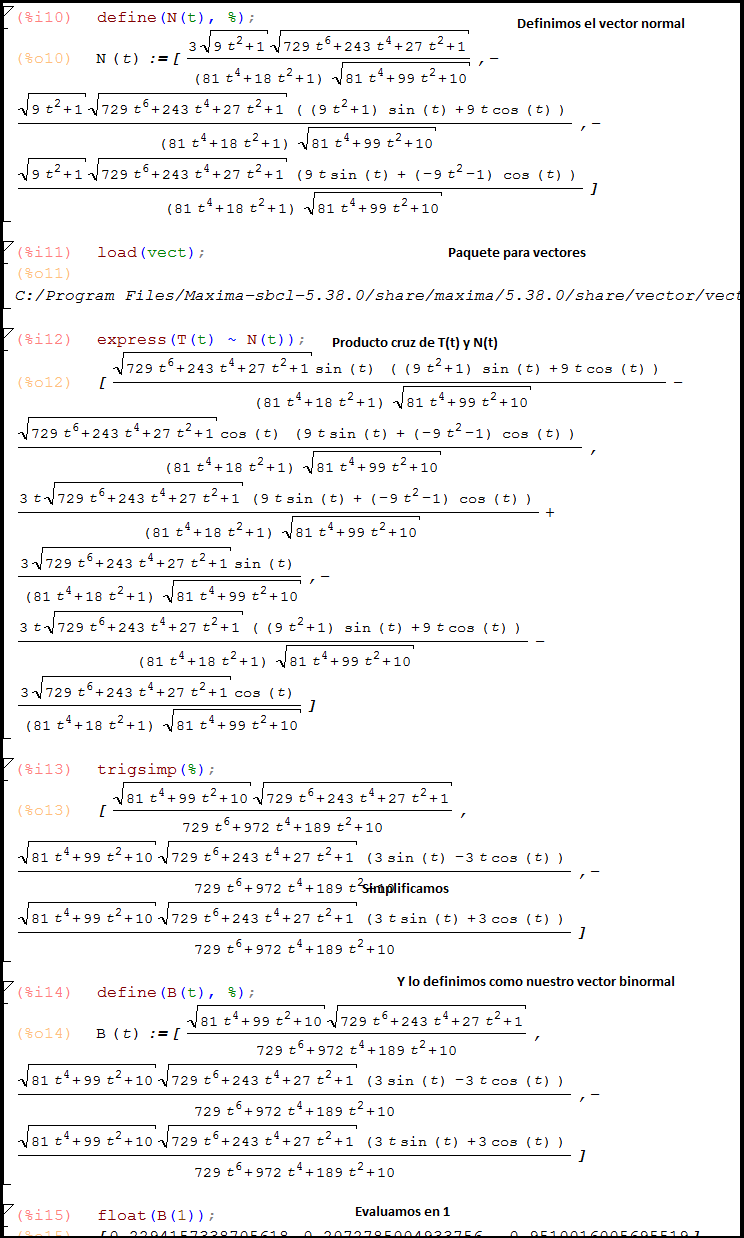
\includegraphics[width=10.4cm, height=16 cm]{VectorBinormal.png}
  \caption{Vector binormal}
\end{figure}

%---------------------------------------------------------------------

\section*{Cap\'itulo 3}
\subsection*{3.1 Funciones de varias variables}

\begin{figure}[!ht]
  \centering
      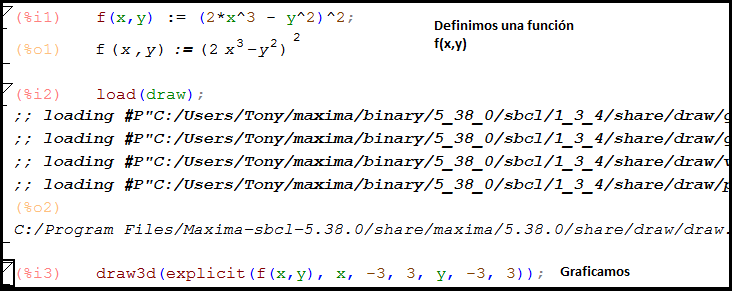
\includegraphics[width=9.0cm, height=4.0 cm]{GraficaCodigo.png}
  \caption{Funci\'on de varias variables}
\end{figure}

\newpage

\begin{figure}[!ht]
  \centering
      \includegraphics[width=9.0cm, height=8.0 cm]{GraficaF_x_y_.png}
  \caption{Gr\'afica de la funci\'on}
\end{figure}

\begin{figure}[!ht]
  \centering
      \includegraphics[width=9.0cm, height=8.0 cm]{GraficaF_x_y_2.png}
  \caption{Gr\'afica de la funci\'on 'enhanced'}
\end{figure}

\begin{figure}[!ht]
  \centering
      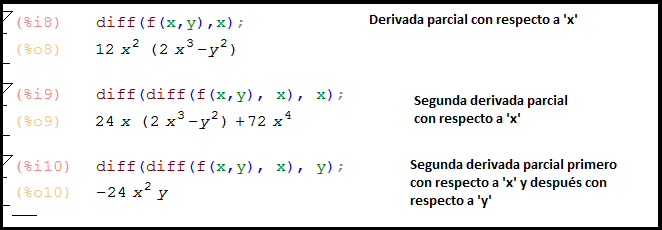
\includegraphics[width=8.0cm, height=3.8 cm]{DerivadasParciales.png}
  \caption{Derivadas parciales de una funci\'on de varias variables}
\end{figure}
\newpage
%------------------------------------------------------------------
\subsection*{3.2 Aproximaciones lineales y diferenciales}

\begin{figure}[!ht]
  \centering
      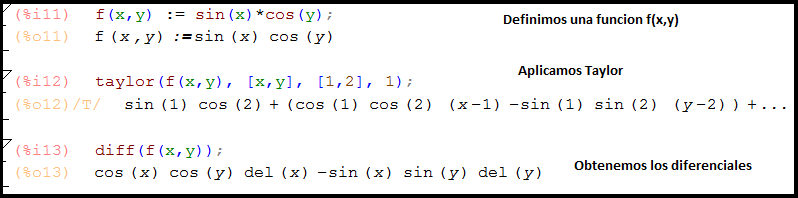
\includegraphics[width=8.0cm, height=2.0 cm]{AproxDiferenciales.png}
  \caption{Aproximaci\'on lineal y diferenciales de una funci\'on de varias variables}
\end{figure}

%---------------------------------------------------------------------
\subsection*{3.3 Regla de la cadena y Derivaci\'on impl\'icita}

\begin{figure}[!ht]
  \centering
      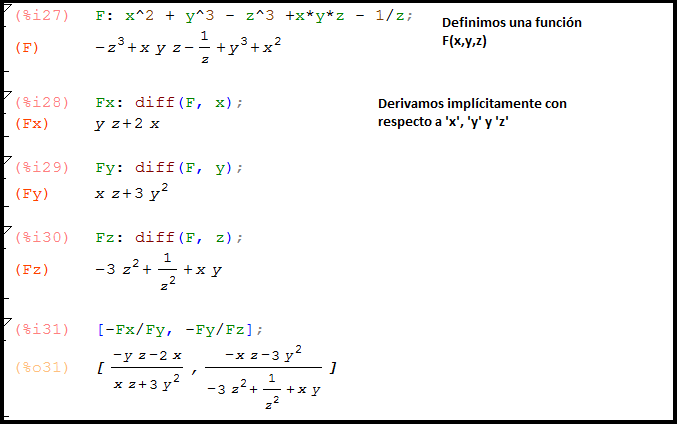
\includegraphics[width=7.0cm, height=4.5 cm]{ReglaCadena.png}
  \caption{Aplicaci\'on de la regla de la cadena a una funci\'on}
\end{figure}

\begin{figure}[!ht]
  \centering
      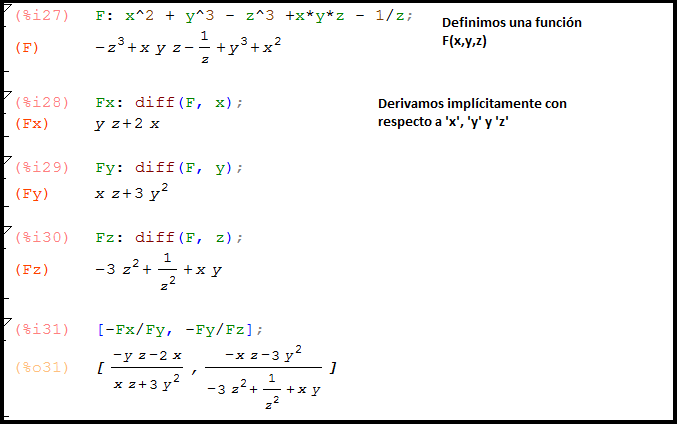
\includegraphics[width=7.0cm, height=4.5 cm]{Implicita.png}
  \caption{Derivadas impl\'icitas de una funci\'on}
\end{figure}

%--------------------------------------------------------------------
\subsection*{3.4 Derivadas direccionales y Gradiente}
\newpage
\begin{figure}[!ht]
  \centering
      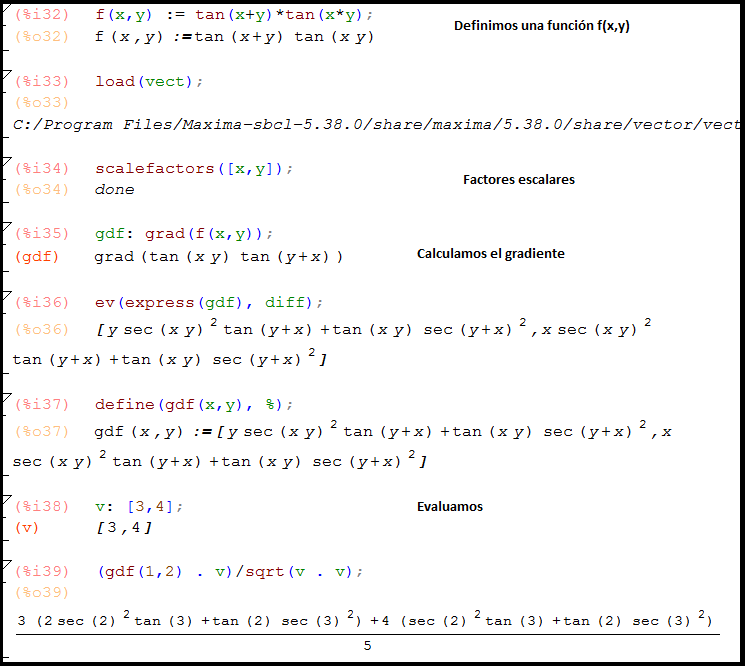
\includegraphics[width=8.0cm, height=7.0 cm]{Gradiente.png}
  \caption{Gradiente y Derivada direccional}
\end{figure}

%---------------------------------------------------------------------

\subsection*{3.5 Optimizaci\'on y extremos locales}

\begin{figure}[!ht]
  \centering
      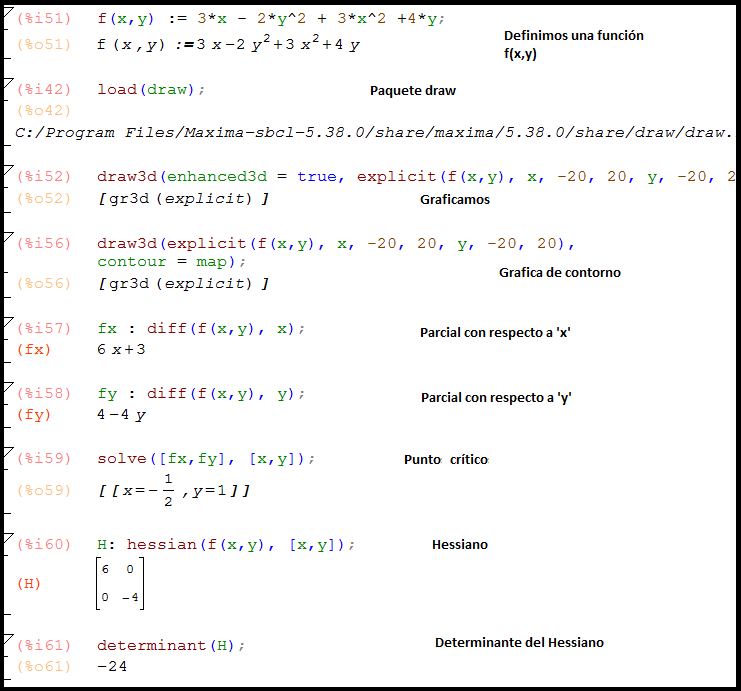
\includegraphics[width=8.0cm, height=7.0 cm]{Optimizacion.png}
  \caption{Optimizacion de una funcion}
\end{figure}

\begin{figure}[!ht]
  \centering
      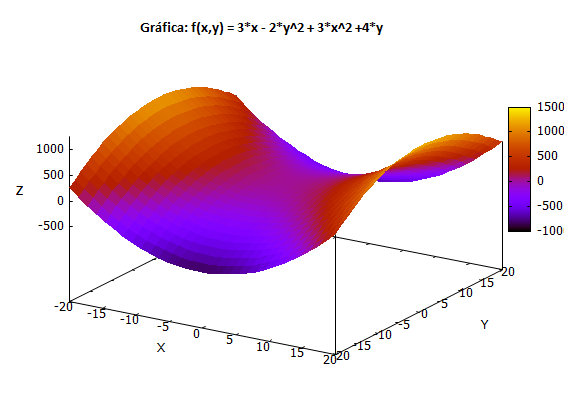
\includegraphics[width=7.0cm, height=5.0 cm]{GraficaOptimizacion.png}
  \caption{Grafica de la funcion}
\end{figure}
\newpage
\begin{figure}[!ht]
  \centering
      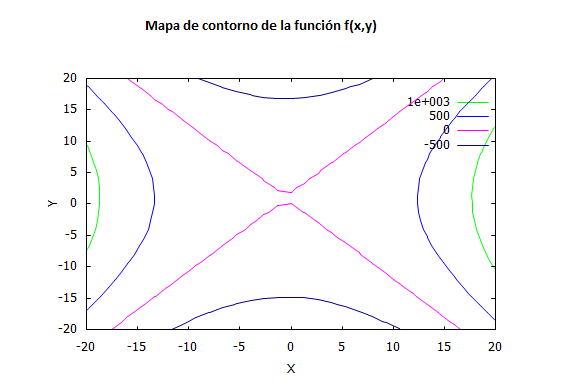
\includegraphics[width=9.0cm, height=8.0 cm]{MapaContorno.png}
  \caption{Mapa contorno}
\end{figure}

%-----------------------------------------------------------------

\section*{Cap\'itulo 4}
\subsection*{4.1 Integrales Dobles}

\begin{figure}[!ht]
  \centering
      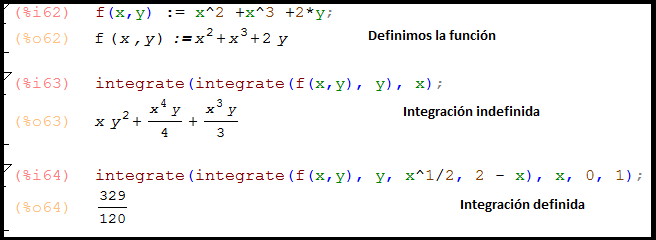
\includegraphics[width=6.5cm, height=2.4 cm]{IntegracionDoble.png}
  \caption{Integraci\'on Doble en Maxima}
\end{figure}

%------------------------------------------------------------------

\subsection*{4.2 Integraci\'on en coordenadas polares}

\begin{figure}[!ht]
  \centering
      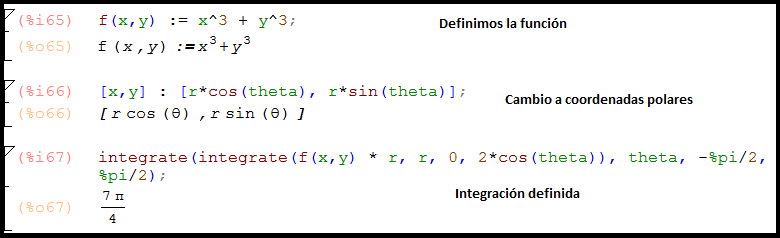
\includegraphics[width=6.5cm, height=2.4 cm]{IntegracionDoblePolares.png}
  \caption{Integraci\'on en coordenadas polares}
\end{figure}

%--------------------------------------------------------------------

\subsection*{4.3 Integrales Triples}

\begin{figure}[!ht]
  \centering
      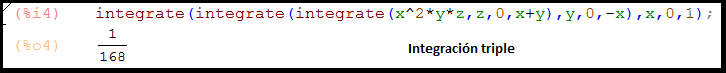
\includegraphics[width=7.2cm, height=1.0 cm]{IntegracionTriple.png}
  \caption{Integraci\'on triple}
\end{figure}

%--------------------------------------------------------------------

\subsection*{4.4 Integrales en coordenadas cil\'indricas y esf\'ericas}

\begin{figure}[!ht]
  \centering
      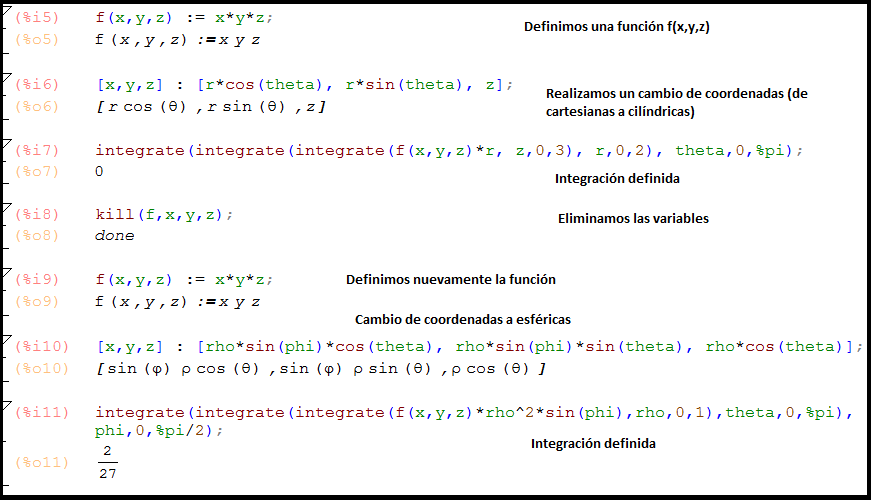
\includegraphics[width=8.7cm, height=5.0 cm]{IntegracionCE.png}
  \caption{Integraci\'on en coordendas cil\'indricas y esf\'ericas}
\end{figure}

%--------------------------------------------------------------------

\subsection*{4.5 Cambio de variables}

\begin{figure}[!ht]
  \centering
      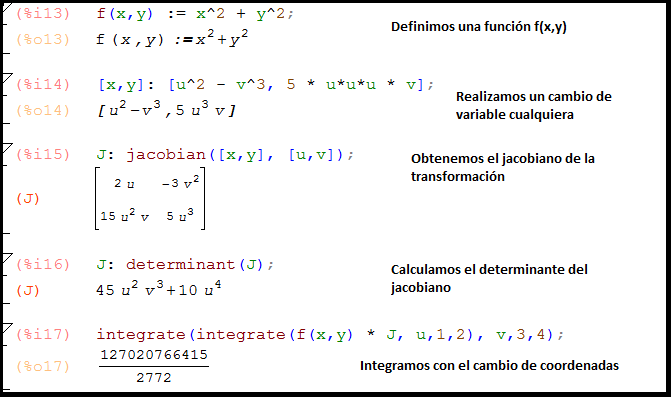
\includegraphics[width=7.0cm, height=4.2 cm]{Jacobiano.png}
  \caption{Jacobiano de la transformaci\'on}
\end{figure}

%_-------------------------------------------------------------------
\section*{Cap\'itulo 5}
\subsection*{5.1 Campos vectoriales}

\begin{figure}[!ht]
  \centering
      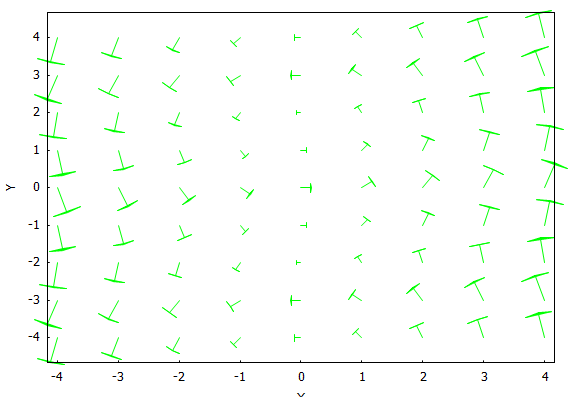
\includegraphics[width=7.0cm, height=6.2 cm]{Campo2D.png}
  \caption{Campo vectorial en 2 dimiensiones}
\end{figure}
\newpage
\begin{figure}[!ht]
  \centering
      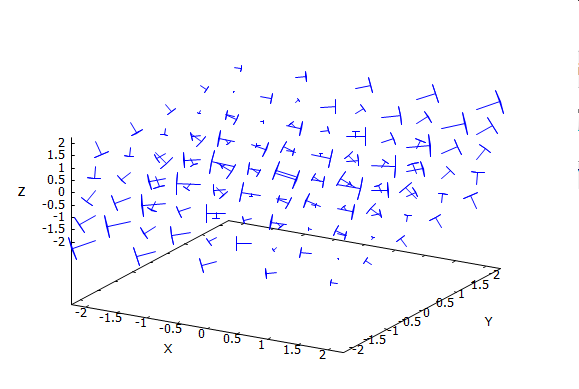
\includegraphics[width=7.0cm, height=6.2 cm]{Campo3D.png}
  \caption{Campo vectorial en 3 dimensiones}
\end{figure}

%-----------------------------------------------------------------

\subsection*{5.2 Integrales de Linea}

\begin{figure}[!ht]
  \centering
      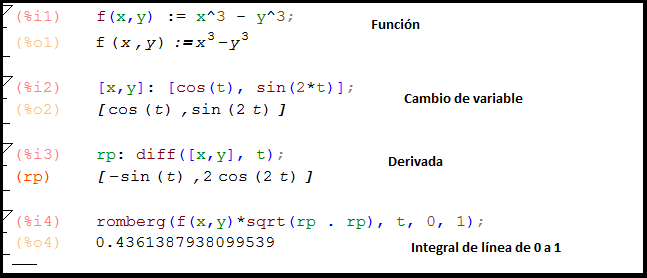
\includegraphics[width=7.0cm, height=3.0 cm]{IntegralLinea.png}
  \caption{Integral de Linea}
\end{figure}

\begin{figure}[!ht]
  \centering
      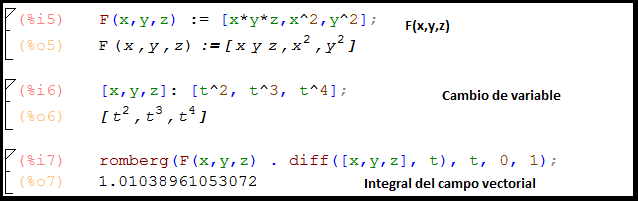
\includegraphics[width=7.0cm, height=3.0 cm]{IntegralLineaVectorial.png}
  \caption{Integral de Linea m\'as general}
\end{figure}

%-----------------------------------------------------------------

\subsection*{5.3 Campos vectoriales conservativos}

\begin{figure}[!ht]
  \centering
      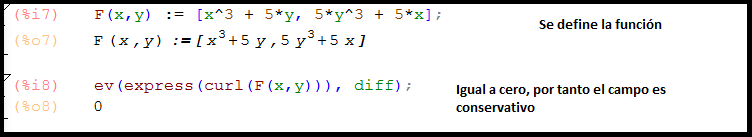
\includegraphics[width=7.0cm, height=2.0 cm]{CampoConservativo.png}
  \caption{Campo vectorial conservativo}
\end{figure}
\newpage
\begin{figure}[!ht]
  \centering
      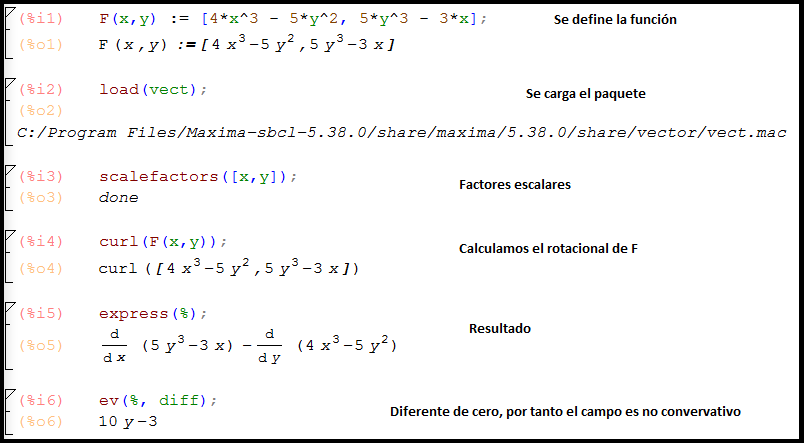
\includegraphics[width=7.0cm, height=6.0 cm]{CampoNoConservativo.png}
  \caption{Campo Vectorial No conservativo}
\end{figure}

\end{document}